\documentclass{article}

\usepackage{graphicx}
\usepackage{tikz}
\usepackage{tikzsymbols}
\usetikzlibrary{calc,patterns,shapes.geometric}
\pagestyle{empty}
\usepackage[margin=0pt]{geometry}
\geometry{papersize={14in,12in}}

\def\centerarc[#1](#2)(#3:#4:#5){\draw[#1] ($(#2)+({#5*cos(#3)},{#5*sin(#3)})$) arc (#3:#4:#5);}

\begin{document}
	\begin{figure}
		\centering
		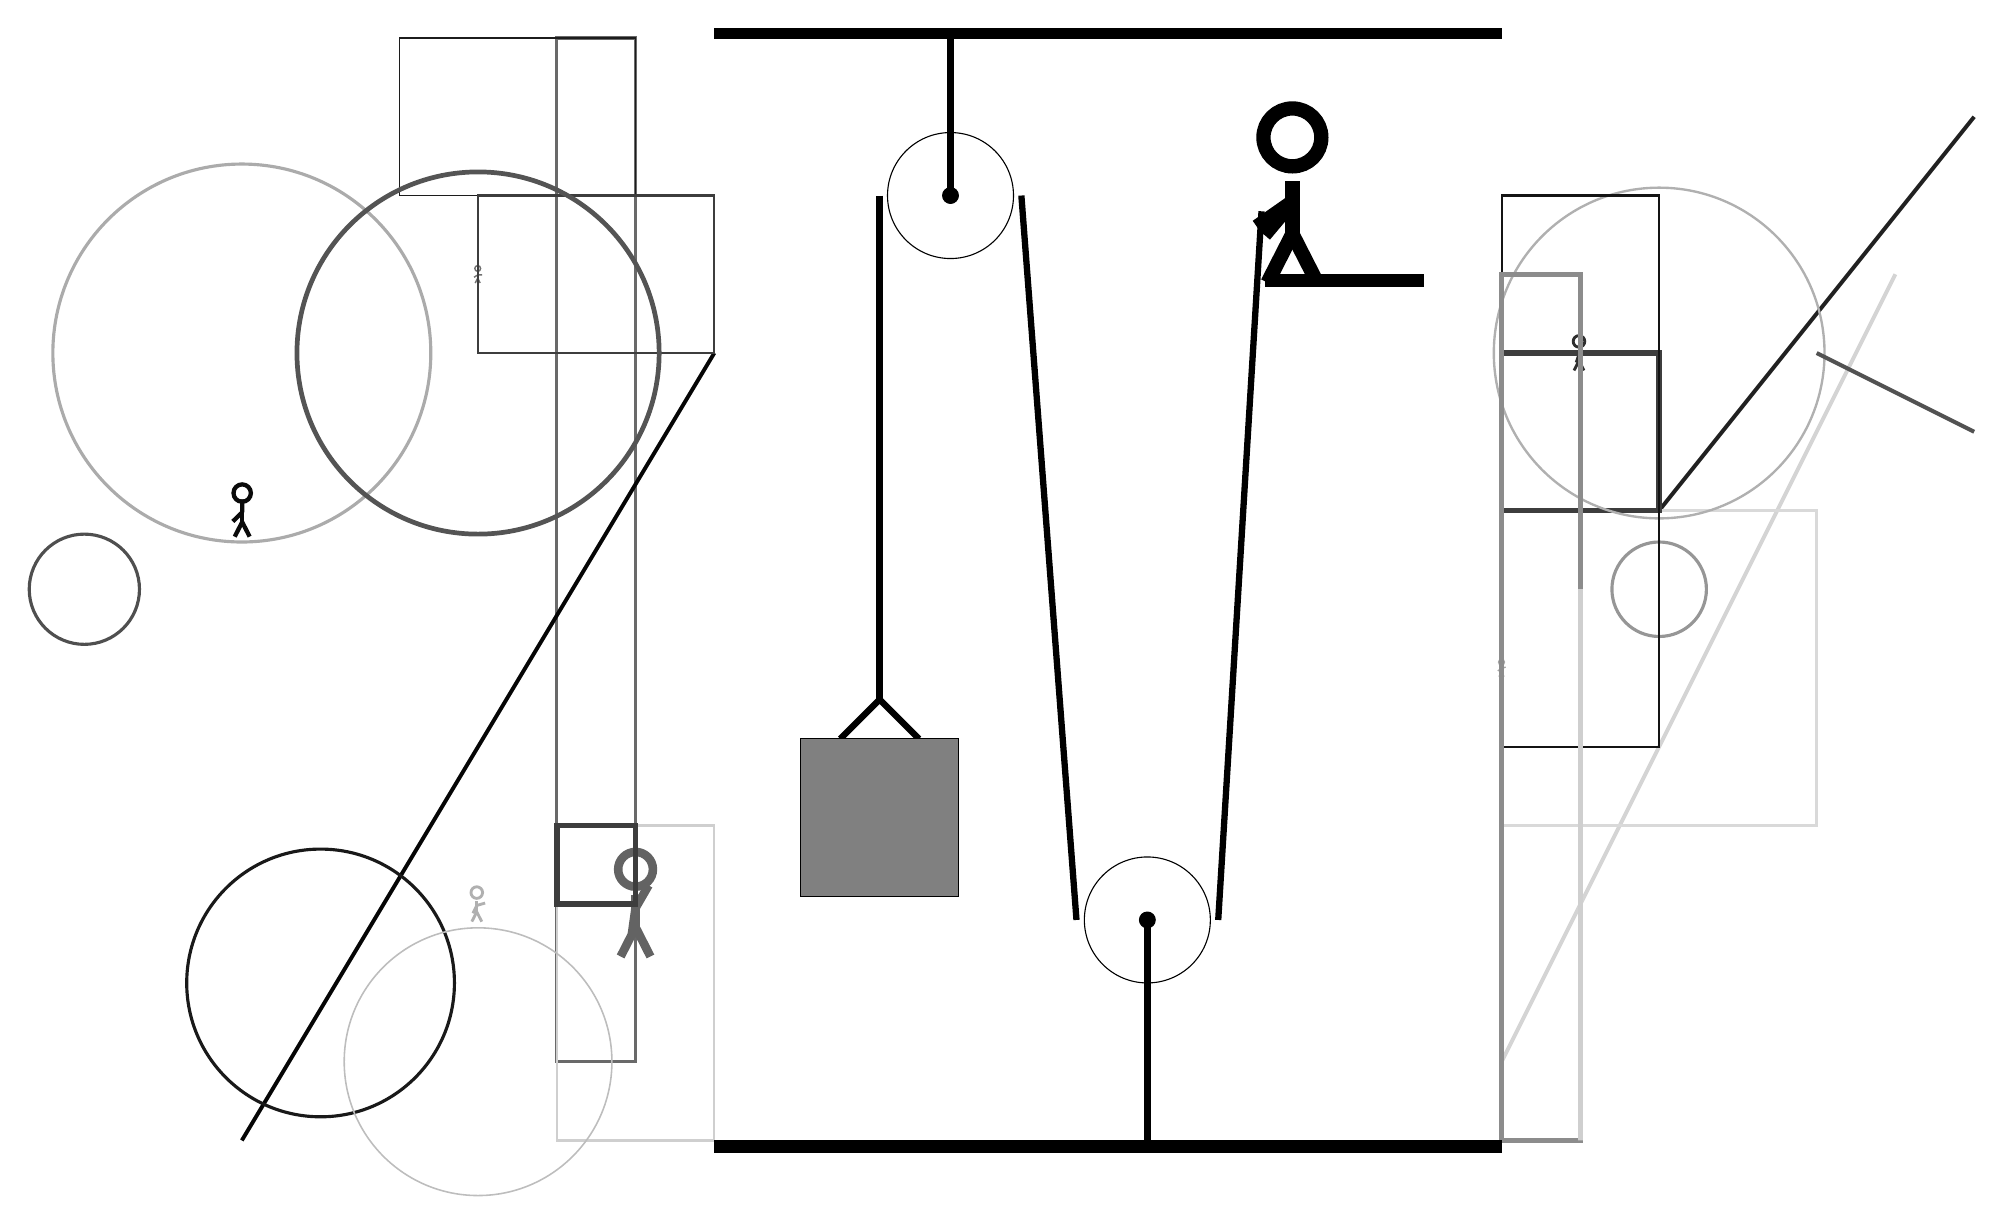
\begin{tikzpicture}
			%%%%% START %%%%%
			
			\draw[fill=black] (-2, 14) rectangle (8, 14.125);
			
			\draw (3.5, 2.8) circle (0.8);
			\draw[fill=black] (3.5, 2.8) circle (0.1);
			\draw[line width=0.8mm] (3.5, 2.8) -- (3.5, 0);
			
			\draw (1, 12) circle (0.8);
			\draw[fill=black] (1, 12) circle (0.1);
			\draw[line width=0.8mm] (1, 14) -- (1, 12);
			
			\draw[line width=0.8mm](-0.4, 5.1) --  (0.1, 5.6) -- (0.6, 5.1);
			\draw[fill=black!50] (-0.9, 5.1) rectangle (1.1, 3.1);
			
			\node[line width=0.3mm, color=black!31] at (-5, 3) {\Strichmaxerl[2][64][16]};
			
			\node[line width=0.2mm, color=black!35] at (8, 6) {\Strichmaxerl[1][31][21]};
			\draw[line width=0.4mm, color=black!59] (-3, 14) rectangle (-4, 1);
			\node[line width=0.3mm, color=black!56] at (-5, 11) {\Strichmaxerl[1][33][1]};
			
			\node[line width=0.2mm, color=black!96] at (-8, 8) {\Strichmaxerl[3][44][89]};
			
			\draw [line width=0.4mm, color=black!41](10, 7) circle (0.6);
			\draw[line width=0.5mm, color=black!17](13, 11) -- (8, 1);
			
			\draw[line width=0.5mm, color=black!87](10, 8) -- (14, 13);
			\node[line width=0.2mm, color=black!82] at (9, 10) {\Strichmaxerl[2][71][6]};
			
			\draw[line width=0.4mm, color=black!15] (8, 4) rectangle (12, 8);
			\draw[line width=0.2mm, color=black!89] (-3, 12) rectangle (-6, 14);
			\draw [line width=0.4mm, color=black!33](-8, 10) circle (2.4);
			\draw[line width=0.5mm, color=black!74](10, 8) -- (10, 10);
			
			\draw[line width=0.7mm, color=black!76] (8, 8) rectangle (10, 10);
			\node[line width=0.4mm, color=black!61] at (-3, 3) {\Strichmaxerl[6][82][60]};
			\draw[line width=0.5mm, color=black!98](-2, 10) -- (-8, 0);
			\draw [line width=0.4mm, color=black!69](-10, 7) circle (0.7);
			\draw [line width=0.4mm, color=black!90](-7, 2) circle (1.7);
			\draw[line width=0.3mm, color=black!19] (-4, 4) rectangle (-2, 0);
			\draw[line width=0.3mm, color=black!76] (-2, 12) rectangle (-5, 10);
			\draw [line width=0.3mm, color=black!31](10, 10) circle (2.1);
			\draw[line width=0.3mm, color=black!92] (8, 12) rectangle (10, 5);
			
			\draw [line width=0.2mm, color=black!26](-5, 1) circle (1.7);
			\draw [line width=0.6mm, color=black!67](-5, 10) circle (2.3);
			\draw[line width=0.5mm, color=black!68](12, 10) -- (14, 9);
			
			\draw[line width=0.7mm, color=black!76] (-4, 4) rectangle (-3, 3);
			\draw[line width=0.7mm, color=black!45] (8, 0) rectangle (9, 11);
			\draw[line width=0.7mm, color=black!19] (9, 0) rectangle (9, 7);
			
			
			\draw[line width=0.8mm](0.1, 12) -- (0.1, 5.6);
			\centerarc[line width=0.8mm](1, 12)(180:0:0.9)
			\draw[line width=0.8mm](1.9, 12) -- (2.6, 2.8);
			\centerarc[line width=0.8mm](3.5, 2.8)(180:360:0.9)
			\draw[line width=0.8mm](4.4, 2.8) -- (4.95, 11.8);
			
			\node at (5.3, 12) {\Strichmaxerl[10][35][-130]};
			\draw[fill=black] (5, 11) rectangle (7, 10.85);
			
			\draw[fill=black] (-2, 0) rectangle (8, -0.15);
			
			%%%%% END %%%%%
		\end{tikzpicture}
	\end{figure}	
\end{document}